\documentclass{article}

\usepackage{graphicx}
\usepackage{amsmath, amssymb}
\usepackage{bm}

\newcommand{\phib}{\bm{\phi}}
\DeclareMathOperator*{\argmax}{arg\,max}

\usepackage{nips12submit_e, times}
\usepackage{hyperref}

\title{An Empirical Study of Approximate Inference Algorithms on Bayesian
Logistic Regression}

\author{
Wei Dai \\
School of Computer Science \\
Carnegie Mellon University\\
Pittsburgh, PA 15213\\
\texttt{wdai@cs.cmu.edu}\\
\And
Abhimanu Kumar \\
School of Computer Science \\
Carnegie Mellon University\\
Pittsburgh, PA 15213\\
\texttt{abhimank@cs.cmu.edu}\\
\And
Jinliang Wei \\
School of Computer Science \\
Carnegie Mellon University\\
Pittsburgh, PA 15213\\
\texttt{jinlianw@cs.cmu.edu}\\
}
\newcommand{\fix}{\marginpar{FIX}}
\newcommand{\new}{\marginpar{NEW}}
\nipsfinalcopy
\begin{document}
\maketitle

\setcounter{page}{1}
\pagenumbering{arabic}
% \vspace{-20pt}
% \section{Project Idea}
% \vspace{-5pt}

Graphical models have been extensively used in recent decades in the
broader research area of machine learning: from linguistics to network discovery and
structure prediction in parsers to online social media~\cite{Koller+Friedman:09}
Graphical models provide a convenient way of  representing complex structures.
They are a great tool to represent data which has an intuitive generative
or a causal story~\cite{GettingStarted}. In most of these cases we are
estimating the parameters of the probabilistic model where some of the member
nodes of the graphs are not observed or hidden. Models like these are also very
useful in the cases when one has a causal story where there are hidden states of
the in the causal chain for e.g. hidden markov model~\cite{Baum1967}. Graphical
modelling is one of the most effective way to estimate models that involve
transitions over a state space e.g. temporal modelling
\cite{Arnold:2007:TCM:1281192.1281203}. There have been various methods
proposed for estimating parameters of such a model. 
there have been a lot of extensive analysis of these models in terms of the
\section{Related Works}

Asuncion {\it et. al.}~\cite{Asuncion2009smoothing} compared several
approximation algorithms for Latent Dirichlet Allocation (LDA), including
variants of variational Bayes, ML estimation, maximum a posterior (MAP), and
collapsed Gibbs sampling. They report that LDA is more sensitive to the
hyperparameters than the approximation algorithms. However, finding optimal
hyperparameters are generally expensive, and they showed that iterative method
(e.g.~\cite{Minka00}) is not always optimal. Due to the nature of LDA, the
study does not yield performance comparison of classification task. Jiang {\it
et. al.}~\cite{medlda_MCMC12} report that sampling-based approximations
significant out-perform variational methods on classification tasks using
max-entropy discrimination LDA (MedLDA), a supervised variant of LDA.
Both~\cite{Asuncion2009smoothing, medlda_MCMC12} use only text corpus, while
our study include text, genomics data, and diseases data (sec.~\ref{sec:experiments}). 

Mukherjee {\it et. al.}~\cite{Mukherjee08} provide a theoretical comparison of
two variational Bayes methods for LDA based on mean-field approximation. Here
we consider Bayesian logistic regression which does not lend to mean field
factorization and thus require potentially more challenging variational
methods. Another comparative study over LDA model is by Wallach et
al.~\cite{WallachMM09} where they study different priors and the
corressponding MAP estimates for LDA. Though they mostly concern with LDA and
priors they do enrich the literature with their valuable analysis and provide
some insights regarding the choice of priors and sampling techniques. 

Holmes et. al~\cite{Holmes} study MCMC estimation techniques over Bayesian logistic
regression in great detail. They build up the bayesian framework for logistic
regression from logit function to all the way upto Kolmogorov-Smirnov prior over
the regression parameter. Since the resultant posterior does not have a nice
closed form, they provide rejection based sampling over set of truncated
normals for the parameter updates. The experiments are performed over resonably
diverse datasets, though the only problem is the low dimension of their
datastes. All of their datasets have dimension less than ten which is way
smaller than a real world dataset. We in our experiments have tried to maintain
a diverse set of datasets which deal in very high deimension space. The
compartive analysis changes in the higher dimension since the sampling
strategies tend to be slower and less accurate as one increases the dimension of
the data. 

As one can see there has not been any substantial works done in the area of
statistics or machine learning for a comparaitive study of various approximate
estimation techniques inclding sampling, variational and Laplace techniques, for
graphical models. Besides we also perform a comparitive study of these
techniques over two distinct graph objectives: 1) MLE, and 2)MAP. It
would be a worthwhile effort which has a potential to provide working insights
into the world of these complex estimation techniques. For Bayesian logistic
regression gibbs sampling is a simplified version of the Metropolis–Hastings
algorithm (\cite{Metropolis53}; \cite{Hastings70}), and is used whenever it is
possible to sample directly from all conditional distributions. The Metropolis–Hastings algorithm
is generally used in the case of logistic regression. Other Markov chain
Monte Carlo techniques in use are adaptive rejection sampling (ARS), which is used in the WinBugs
software, and adaptive rejection metropolis sampling (ARMS).



\section{Methods}

\begin{figure}[t]
\centering
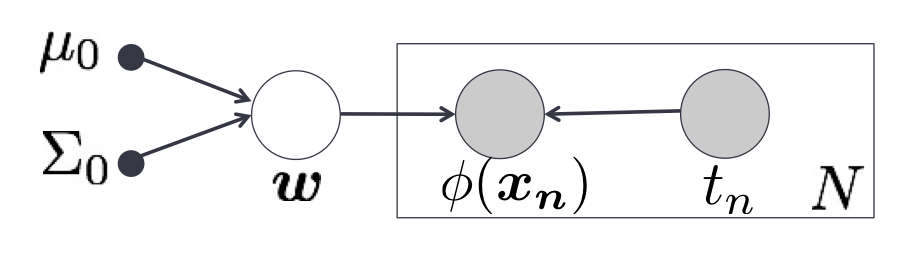
\includegraphics[height=3.0cm]{BLR_graphical.png}

\caption{\small Graphical model of Bayesian logistic regression. Here
$t_n \in \{0,1\}$ is the class label, $\phi({\bf x}_n)$ is the feature map,
and ${\bf w}$ is the model parameter.}

\label{fig:BLR_graphical}
\end{figure}

Given data set $\{\phib_n, t_n\}_{n=1}^N$ where $\phib_n$ are the feature
vectors and $t_n\in \{0,1\}$ are the labels, we can write the likelihood
function for logistic regression as $p(\bm{t}|\bm{w}) = \prod_{n=1}^N
y_n^{t_n} (1-y_n)^{1-t_n}$ where $\bm{t} = (t_1,...,t_N)^T$ and
$y_n=p(\mathcal{C}_1|\phib_n) = \sigma(\bm{w}^T \phib_n)$ and $\sigma(s) =
\frac{1}{1+e^{-s}}$. Using Bayes rule, the posterior distribution over
$\bm{w}$ is $p(\bm{w}|\bm{t}) = \frac{p(\bm{w}) p(\bm{t}|\bm{w})}{p(\bm{t})}$
where $p(\bm{t}) = \int p(\bm{w})p(\bm{t}|\bm{w}) d\bm{w}$ involves logistic
sigmoid functions and is intractable. In the sequel we briefly describe three
approximation schemes (Laplace approximation, variational methods, and Gibbs
sampling), and point estimations (MLE, MAP) together with the associated
prediction rules.

\subsection{Markov Chain Monte Carlo approximation}
\label{sec:MCMCmethod}
Let us first discuss the simple bayesian binary probit regression model and 
then we will ease into bayesian logistic regression. We follow the lead of
the work done by Holmes et al.~\cite{Holmes}. Let $\psi$ denotes the gaussian
cdf, binary probit regression's likelihood is:
\begin{equation}
\pi(y_i=1|x_i) = \psi(x_i^Tw)
\end{equation}

We define a set of n auxiliary variables $z_i$ as there is no cojugate prior to
the gaussian cdf as:
\begin{equation}
z_i=x_i^Tw+\epsilon_i
\end{equation}

and $\epsilon_i \sim N(0,1)$, and if $z_i>0$ then $y_i=1$ and vice-versa.
Removing w from likelihood in this new model makes the model more amenable
to sampling. For this
specific case of  Normal prior over w, this model has a simple
Gibbs sampling updates where $z_i$ is drawn from independent 
truncated Normal distributions, and w is drwn from a multvariate Normal
distribution. Formally, a easy-to-follow Gibbs sampling scheme with
$\pi(w)\sim N(b,v)$ can be obtained using the following:
\begin{eqnarray}
z_i|w \propto N(x_i^Tw,1)I(z_i>0)y_i=1 \\
z_i|w \propto N(x_i^Tw,1)I(z_i\leq 0)y_i\neq 0 \\
w|z,y \sim N(B,V) \\
B = V(v^{-1}b+X^Tz) \\
V=(v^{-1}+X^TX)^-1 \\
\end{eqnarray}

This simple Gibbs sampling strategy is poor in performance because the
components of w are strongly correlated with the components of z. To remove this
we sample w and z together through the use of the product rule:
\begin{equation}
\pi(w,z|y) = \pi(z|y)*\pi(w|z)
\end{equation}

This method draws every $z_i$ from a Normal distribution that has means
and variances obtained using a leave-one-out marginal predictive density,
and these conditional means are updated after each draw of $z_i$.
Later we sample w from its conditional gaussian after all of the
$z_i$ have been drawn. 

\subsubsection{Binary Logistic Regression}
Starting from the binary Bayesian probit regression model explained before , we
propose to obtain updates for binary Bayesian logistic regression by
substituting the independent Normal 
prior over $\epsilon$ with independent logistic. 
This significantly alters the simple sampling scheme we described earlier. To
obtain a simple sampling strategy of the new model we define an addtional group
of auxiliary variables $λ_{1:n}$ along side modifying the noise function to get
a scale mixture of gaussians with marginal densities as logistic distribution,
(here KS is the Kolmogorov-Smirnov distribution):
\begin{eqnarray}
\epsilon_i \sim N(0,\lambda_i) \\
\lambda_i = (2\nu_i)^2 \\
\nu_i \sim KS \\
\end{eqnarray}

If one takes $\lambda$ to be  constant, then this is identical to the
Probit model above. Though each value of $z_i$ contains an individual term i for
its noise variance now. Moreover, the greatest advantage is that we know the way
to draw samples from this model given fixed $\lambda$ . We just have to use
weighted least squares rather than least squares (and teh related inverse of the 
hessian matrix), and then just draw from individual truncated gaussain of
different variance parameters. After this, we are in a poition to write a
Gibbs sampler given that we will be able to sample from the KS distribution.
\cite{Holmes} provides rejection sampling technique to draw samples 
from the KS distribution via the Generalized Inverse Gaussian distibution as the
sampling density. Using this, we write a simple Gibbs sampler for this
logistic regression setting as follows:

\begin{eqnarray}
z_i|w,\lambda \propto N(x_i^Tw,\lambda_i)I(z_i>0)~if~y_i=1 \\
z_i|w,\lambda \propto N(x_i^Tw,\lambda_i)I(z_i\leq 0)~if~y_i\neq 0 \\
w|z,y.\lambda \sim N(B,V) \\
B = V(v^{-1}b+X^TWz) \\
V=(v^{-1}+X^TWX)^{-1} \\
W=diag(\lambda^{-1}) \\
\end{eqnarray}

\subsection{Laplace Approximation and associated MAP}

Laplace approximation approximate the posterior $p(\bm{w}|\bm{t})$ with a
multivariate Guassian $\mathcal{N}(\bm{w}; \bm{w}_{MAP}, \bm{S}_N)$ where
$\bm{w}_{MAP}$ is the maximum {\it a posteriori} and thus a mode of the
posterior and $\bm{S}_N^{-1} = -\nabla^2_{\bm{w}} \ln
p(\bm{w}|\bm{t})|_{\bm{w} = \bm{w}_{MAP}}$ is the Hessian at $\bm{w}_{MAP}$.
Since we are approximating the posterior with Gaussian, it is convenient to
use conjugate prior $p(\bm{w}) = \mathcal{N}(\bm{w};\bm{m}_0,\bm{S}_0)$. Thus
we have $\ln p(\bm{w}|\bm{t}) = -\frac{1}{2}(\bm{w}-\bm{m}_0)^T
\bm{S}_0^{-1}(\bm{w}-\bm{m}_0) + \sum_{n=1}^N\{t_n \ln y_n +(1-y_n) \ln
(1-y_n)\} + const$

Under the Laplace approximation and the conjugated Gaussian prior, $\bm{w}_{MAP}$
can be efficiently obtained by gradient descent. To encourage small
$||w||^2_2$, let $\bm{m}_0 = \bm{0}$, and $\bm{S}_0 = \sigma^2 \bm{I}$, we
have the following gradient descent rule: 

\begin{equation}
\bm{w}_t \leftarrow \bm{w}_{t-1} + \eta\left( \sum_{n=1}^N (t_n - y_{n,(t-1)}) \phib_n -
\frac{1}{\sigma^2}\bm{w}_{t-1} \right)
\end{equation}

where $\eta$ is the learning rate constant. We can also get

\begin{equation}
\bm{S}_N^{-1} = -\nabla^2_{\bm{w}} \ln p(\bm{w}|\bm{t})
= \bm{S}_0^{-1} + \sum_{n=1}^N y_n(1-y_n) \phib_n \phib_n^T
\end{equation}

The predictive distribution for Laplace-approximated posterior is not close
form, but by approximating the logistic sigmoid function with probit function,
we recover $\bm{w}_{MAP}$ as the decision boundary.

\subsection{The Variational Approach by Jaakkola and Jordan}
We study a variational method presented by Jaakkola et al.\cite{Jaakkola96avariational}. In this section, we briefly describe the variational method for approximate inference for Bayesian logistic regression. The description closely follows Jaakola's paper.

Since it is infeasible to compute the posterior $p(\bm{w} | \bm{t}, \bm{\phi})$ exactly, this method approximates the sigmoid function with its variational form, as given below.

\begin{align}
  p(t | \bm{w}, \phi) &= \sigma(\Phi_s) \leq \sigma(\xi) exp\{(Phi_s - \xi)/2 + \lambda(\xi)(\Phi_s^2 - \xi^2)\} \\
  &= P(t | \bm{w}, \phi, \xi)
\end{align}
where $\Phi_s = (2t - 1)\sum_jw_j\phi_j$ and $\lambda(\xi) = [1/2 - \sigma(\xi)]/(2\xi)$.

The posterior $P(\bm{w}|\bm{t}, \bm{\phi})$ can be computed by normalizing the left hand side of the following equation.
\begin{align}
\label{eq:variational}
p(\bm{t}|\bm{\phi})p(\bm{w}) &\leq P(\bm{t}|\bm{\phi}, \bm{w}, \xi)P(\bm{w})
\end{align}

Since this normalization is not feasible in practice we normalize the variational distribution instead. As the prior distribution is a Gaussian, we assume it has mean $\mu$ and covariance matrix $\Sigma$. To compute the variational posterior, first, we absorb the observations to update $\mu$ and $\Sigma$.

For each observation, $Sigma$ and $\mu$ are updated as below: 
\begin{align}
\label{eq:sigma_update}
\Sigma^{-1}_{post} &= \Sigma^{-1} + 2|\lambda(\xi)|\phi\phi^T\\
\label{eq:mu_update}
\mu_{post} &= \Sigma_{post}[\Sigma^{-1}\mu + (t - 1/2)\phi]
\end{align}
where $\phi = [\phi_1 ...\phi_n]^T$. 

Now, the posterior covariance matrix depends on the variational parameter $\xi$ through $\lambda(\xi)$ and thus its value needs to be obtained. We obtain $\xi$ by optimizing the approximation in eq. (\ref{eq:variational}). A fast EM algorithm is devised to perform this optimization. This leads to a closed form update for $\xi$. For each observation, the update equation is given by 
\begin{align}
\label{eq:xi}
\xi^2 = E\{(\sum_jw_j\phi_j)^2\} &= \phi^T\Sigma_{post}\phi + (\phi^T\mu_{post})^2
\end{align}

where the expectation is taken with respect to $P(\bm{w}|\bm{\phi}, \xi^{old})$, the variational posterior distribution based on the previous vaue of $\xi$. Alternating between eq. (\ref{eq:sigma_update}), eq. (\ref{eq:mu_update}) and eq. (\ref{eq:xi}) monotonically improves the posterior approximation of eq. (\ref{eq:variational}).

Let $\mathcal{D}$ be the set of all observations. The predictive likelihoods $P(t^p | w_p, \mathcal{D})$ for any complete observation $D^t$ is given by
\begin{align}
  logP(t^p|w_p, \mathcal{D}) = log(\xi_p) - \xi_p/2 - \lambda(\xi_p)\xi_p^2 - \frac{1}{2}\mu^T\Sigma^{-1}\mu + \frac{1}{2}\mu^T_t\Sigma^{-1}_t\mu_t + \frac{1}{2}log\frac{|\Sigma_t|}{|\Sigma|}
\end{align}
where $\mu$ and $\Sigma$ signify the parameters in $P(\bm{w})$ and the subscript $p$ refers to the posterior $P(\bm{w}|\mathcal{D}, D^p)$ found by absorbing the evidence in $D^p$.

We implemented this algorithm, mainly the updating rules in eq. (\ref{eq:sigma_update}), eq. (\ref{eq:mu_update}) and eq. (\ref{eq:xi}). The main advantage of this algorithm is that it usually converges in only 2 to 3 iterations. Although the computation involves expensive matrix inversion, matrix inversion here can be computed as solving a linear system. Therefore, this approach is still pretty fast.

\subsection{Delta Method}



\section{Experiments}
\label{sec:experiments}

\subsection{Data Sets}

We evaluated our implementations of various algorithms on 3 diverse datasets. The feature sets include real numbers, intergers and categorical values. The datasets are randomly split into training sets $80\%$ and
testing sets $20\%$. For multi-class data sets we do one-vs-all (OVA)
classifiers. For approximations that has reasonable run time, we will perform
cross-validation to select parameters for prior, which may have profound
impact on the result as suggested by~\cite{Asuncion2009smoothing}. Details of each dataset can found in Table~\ref{tb:datasets}.

\begin{table}
\begin{tabular}{| c | c |  c | c | c |}
  \hline
  Datasets & \# training instances & \# test instances & \# features & class-wise split\\
  \hline
  Yeast & 1500 & 917 & 103 & (14 classes) \\
  \hline
  Spambase & 3680 & 921 & 57 & 39\% vs. 61\% \\
  \hline
  Heart Diseases & 216 & 54 & 13 & 44\% vs. 56\% \\
  \hline
\end{tabular}

\caption{Datasets information}
\label{tb:datasets}
\end{table}

\subsection{Results}

We compare classification accuracy and run-time of different algorithms. Results are shown in Fig~\ref{fig:results}.

The top graph shows the comparision of different algorithm's classification accuracy. First, we observe that the sampling algorithm outperforms all variational-based approaches on all datasets. However, this does not conclude we should always choose sampling algorithm for better accuracy. Sampling based algorithm suffers when the dimensionality of the data is high. Second, we observe that Delta method performs 


\begin{figure}[t]
\label{fig:results}
\centering
%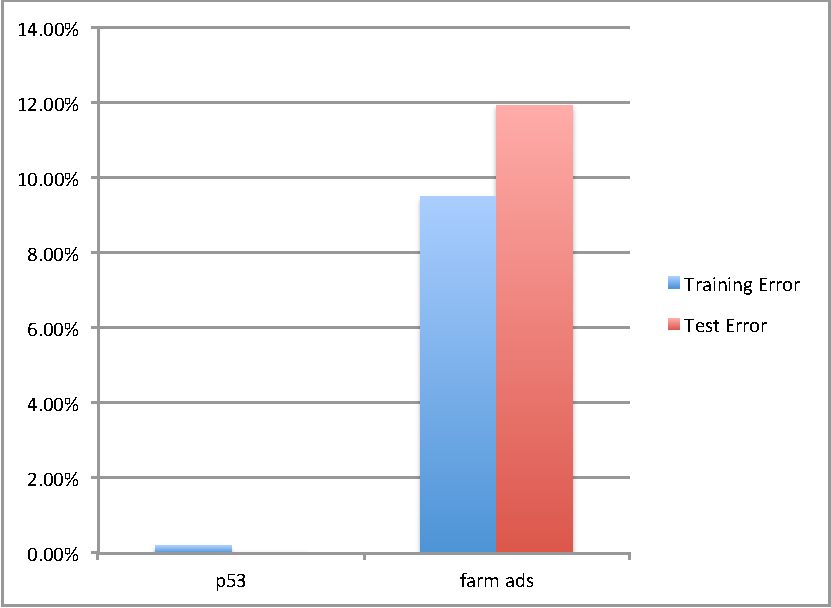
\includegraphics[height=5.0cm]{../../results/classificaiton_errors.pdf}
%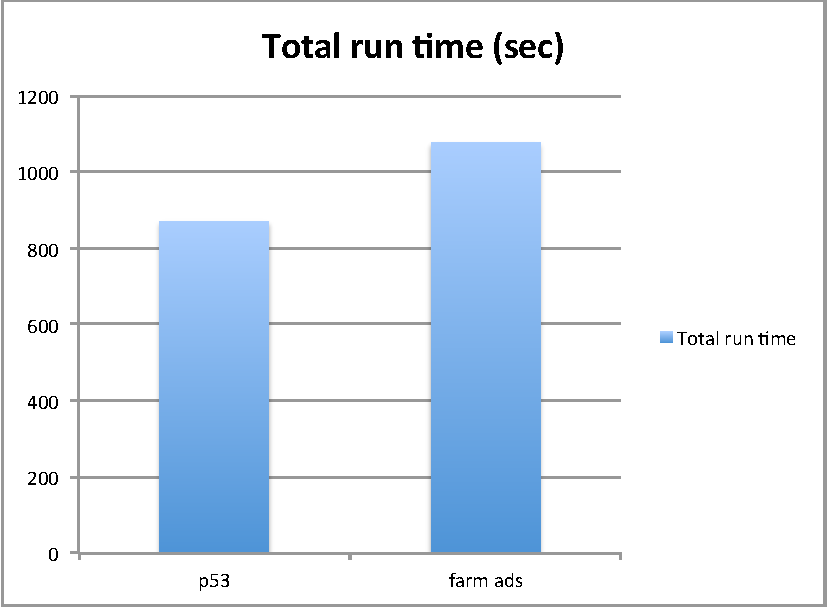
\includegraphics[height=5.0cm]{../../results/runtime.pdf}
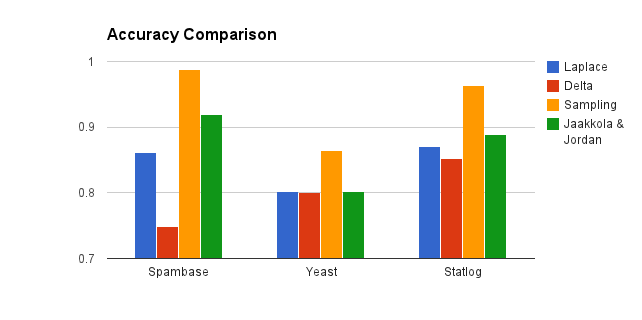
\includegraphics[height=7.0cm]{results/accuracy_comp.png}
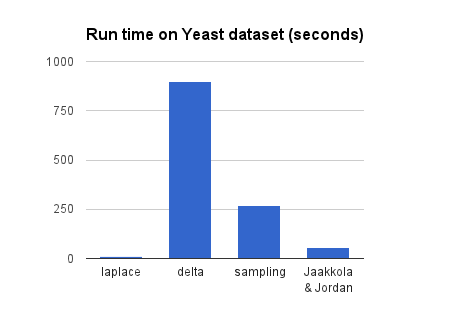
\includegraphics[height=8.0cm]{results/speed_comp.png}

\caption{\small Experiment results; {\bf Top:} Classification accuracy of all algorithms on
four datasets. {\bf Bottom:} Training time for each algorithm on Yeast dataset. }

\label{graphlab}
\end{figure}

\subsubsection{MCMC based estimation}
Our MCMC sampling strategy that we described in section~\ref{sec:MCMCmethod}
converges. Figure~\ref{fig:MCMCconverge} is a plot of the iterations of the Markov 
chain for estimation on a subset of Farms Ads dataset. This is for MLE
estimation without any priors. The X-axix of the figure represents the number of
iteration in sampling and Y-axi si the loglikelihood of theregression model We
also achieve a training accuracy of 8.57\% and a test accuracy of 9.12\% over 
this subset of datset. 

We were only able to run the experiments on this subset of the dataset as the
sampler if slow since we have a rejection sampling component besides various
other samplers. The acceptance ratio of the rejection step is is one quarter on
an average accross number of iterations. In future we plan to fins a better
alternative to this rejection sampler to achieve better speed. 

\begin{figure}[hbt]
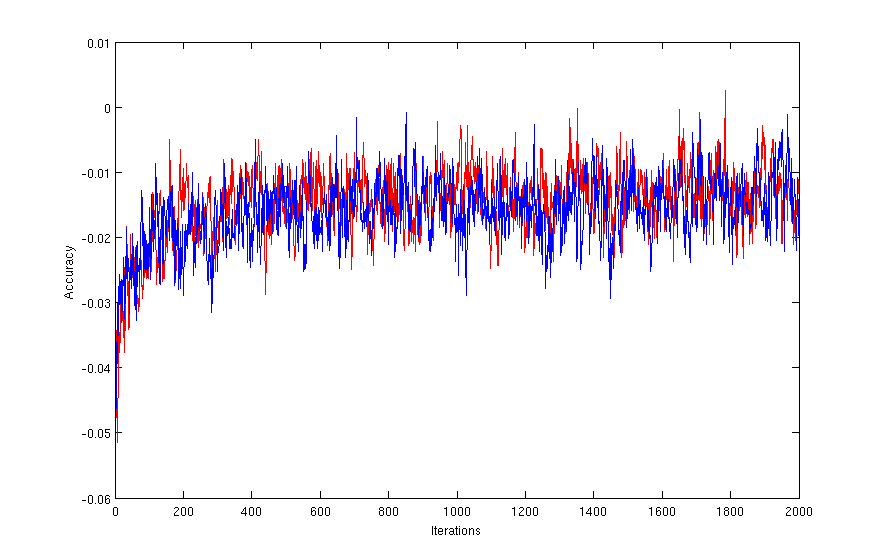
\includegraphics[width=1\textwidth]{results/KSsampleChain.png}
\caption{Two Markov chains (red and blue) converge on the same set of
parameters on the spambase dataset. The
X-axis is the number of iterations and Y-axis is the loglikelihood.}
\label{fig:MCMCconverge}
\end{figure}


\section{Conclusion}



% Latent variable models have gained significant popularity due to their ability to
%  model data that potentially arise due to latent causes. These models are also
%   helpful in case of missing data as these missing entries can be modelled via 
%   hidden variables in graphical models. The parameter estimation for this class 
%   of models are in general intractable, and numerous approximation algorithms 
%   are widely employed. These approaches fall broadly into two categories: 1) 
%   variational inference, and 2) sampling-based. While it is generally believed 
%   that sampling produces better approximation than variational inference, albeit 
%   at a higher computational cost, to the best of our knowledge there is no 
%   comprehensive empirical study that compares these approximation inference schemes.
% 
% We plan to carry out an empirical comparative study of these approximation 
% algorithms on Bayesian logistic regression, a well-studied minimal model with 
% only one latent variable: the regression coefficients. The approximation 
% algorithms we will use are:
% \vspace{-5pt}
% \begin{enumerate}
%   \item Variational inference \cite{RePEc:bes:jnlasa:v:105:i:489:y:2010:p:324-335}:
%     \begin{enumerate}
%       \item A (near) close-form variational bound \cite{Jaakkola96avariational}
%       \item Laplace variational inference and delta method variational 
%       inference \cite{2012arXiv1209.4360W}
%     \end{enumerate}
%     \item Sampling-based: MCMC using Gibbs sampling
% \end{enumerate}
% \vspace{-5pt}
% We would apply the above approximation algorithms to the following estimation 
% problems for a comparative study:
% \vspace{-5pt}
% \begin{enumerate}
%   \item Maximum a posteriori (MAP) from variational and sampling algorithms
%   \item Maximum likelihood estimation (MLE)
%   \item Laplace approximation
% \end{enumerate}
% \vspace{-5pt}
% \section {Software, Datasets and Midterm Milstone}
% \vspace{-5pt}
% We plan to write all the code in matlab or C++ so that we have language agnostic 
% comparison results. We will use 5 
% \href{http://archive.ics.uci.edu/ml/datasets.html}{UCI classification datasets}: 
% 1) Farms Ads dataset (4,143 instances, 54,877 text features), 2) Amazon Commerce 
% reviews dataset (1,500 instances, 10,000 real features) 2) p53 Mutants dataset 
% (16,772 instances, 5,409 real attributes) 4) Human Activity Recognition using 
% Smartphones dataset (10,299 instances, 561 real features) 5) URL Reputation 
% dataset (2,396,130 instances, 3,231,961 real features).
% 
% We plan to finish MCMC sampling for all the three estimation by midterm.
% 
% See reference for papers to read.

\bibliographystyle{plain}
\bibliography{reference}

\end{document}
